\section{Experimental setup}

\begin{figure}[htb]
  \centering
  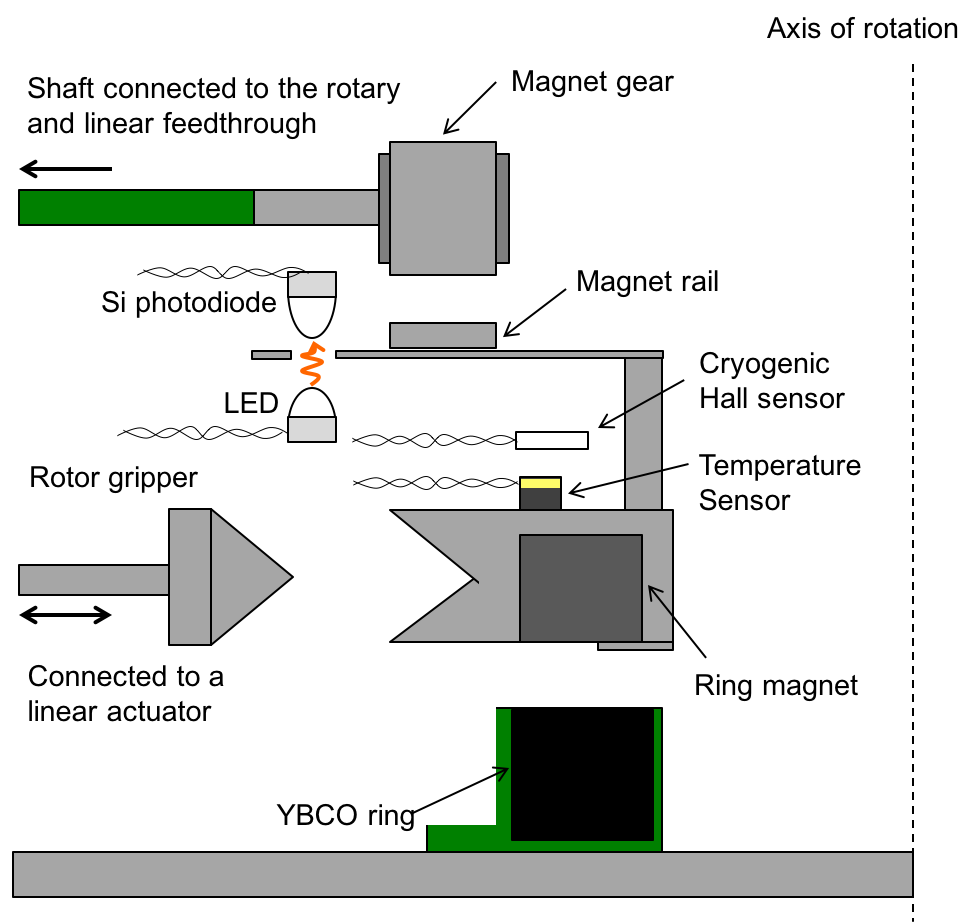
\includegraphics[width=70mm]{../figs/XsecView.eps}%
  \caption{The schematic cross-sectional view of the prototype rotation mechanism.}
  \label{fig:XsecView}
\end{figure}

Fig. X shows cross section view of SMB experimental setup,
which is mainly constructed with a rotor, a stator and a rotor holding system.
The rotor is a NdFeB Permanent Magnet ring (PM) with 1.1 Tesla remnants,
inserted into aluminum frame.
The stator is a YBCO superconductor ring type array with critical temperature of more than 90K,
refrred to as a High Temperature Superconducting (HTS).
As the holding system, three holder arms with cryogenic stepping motors are mounted
to hold the rotor in place above the critical temperature of the HTS.

\begin{itemize}
\item inside including the SMB
\item hall sensor and temperature sensor
\item temperature sensor accuracy
\item DAQ
\end{itemize}
